\documentclass{article}
\usepackage{lambdatex}
\usepackage{tasks}
\usepackage{exsheets}
\newcommand{\se}{\text{ se }}
\renewcommand{\phi}{\varphi}
\everymath{\displaystyle}
\renewcommand{\binom}[2]{\begin{pmatrix}#1\\#2\end{pmatrix}}
\newtheorem*{principio}{Principio}

\usepackage{circuitikz}
\theoremstyle{plain}

\title{Appunti di  Fisica Generale 1\\{\small Primo modulo}}
\author{Davide Borra}
\date{}
\begin{document}
\begin{titlepage}
    \maketitle
    \tableofcontents
    \creativecommons
\end{titlepage}
%\setlength{\headheight}{30pt}
\lhead{Davide Borra}
\rhead{mod. 1}
\chead{Appunti di Fisica Generale 1}
%%%%%%%%%%%%%%%%%%%%%%%%%%%%%%%%%%%%%%%%%%%%%%%%%%%%%
\section{Cinematica del punto materiale}
\subsection{Definizioni preliminari}
\begin{boxdef}[Punto materiale]
    Corpo di dimensioni trascurabili rispetto a quelle dello spazio in cui si muove e di altri oggetti con cui interagisce, le sue dimensioni lineari sono piccole rispetto alla precisione con cui ci interessa determinarne la posizione.
\end{boxdef}
\begin{boxdef}[Gradi di libertà]
    Numero di parametri tra loro indipendenti che servono ad individuare in modo univoco la posizione di un sistema fisico.
\end{boxdef}
\begin{boxdef}[Traiettoria]
    Luogo dei punti occupati successivamente dal corpo puntiforme e che danno origine ad una curva continua nello spazio.
\end{boxdef}
\begin{boxdef}[Vettore posizione]
    Il vettore posizione è quel vettore applicato all’origine del sistema cartesiano scelto, e che ha come estremo libero la posizione del punto $P$.
\end{boxdef}
\subsection{Grandezze fisiche per la cinematica}
Siccome la velocità cambia nel tempo si definiscono due grandezze
\subsubsection{Velocità}
\begin{boxdef}[Velocità media]
    Si definisce velocità media il vettore 
    \[\langle\vec{v}_{(t_1,t_2)}\rangle=\frac{\vec{r}(t_2)-\vec{r}(t_1)}{t_2-t_1}\]
    Essa si misura in ${m}/{s}$
\end{boxdef}
\begin{boxdef}[Velocità istantanea]
    Si definisce velocità istantanea il vettore
    \[\vec{v}(t)=\lim_{t'\to t}\langle\vec{v}_{(t,t')}\rangle=\lim_{t'\to t}\frac{\vec{r}(t')-\vec{r}(t)}{t'-t}= \frac{d \vec{r}}{d t}\]
    Essa si misura in ${m}/{s}$
\end{boxdef}
Siccome per $\Delta t\to 0$ la lunghezza della retta secante approssima la traiettoria sempre meglio, si può affermare che 
\[v(t)=\frac{ds}{dt}\]
\subsubsection{Accelerazione}
Siccome anche l'accelerazione cambia nel tempo si definiscono due grandezze
\begin{boxdef}[Accelerazione media]
    Si definisce accelerazione media il vettore 
    \[\langle\vec{a}_{(t_1,t_2)}\rangle=\frac{\vec{v}(t_2)-\vec{v}(t_1)}{t_2-t_1}\]
    Essa si misura in ${m}/{s^2}$
\end{boxdef}
\begin{boxdef}[Accelerazione istantanea]
    Si definisce accelerazione istantanea il vettore
    \[\vec{a}(t)=\lim_{t'\to t}\langle\vec{a}_{(t,t')}\rangle=\lim_{t'\to t}\frac{\vec{v}(t')-\vec{v}(t)}{t'-t}= \frac{d \vec{v}}{d t}\]
    Essa si misura in ${m}/{s^{2}}$
\end{boxdef}
\begin{boxdef}[Moto rettilineo e moto uniforme]
    Un moto si definisce \textbf{rettilineo} se il versore velocità $\hat{v}$ non cambia (la traiettoria è una retta) e \textbf{uniforme} se il modulo del vettore velocità $|\vec{v}|$ non cambia.
\end{boxdef}

\subsection{Coordinate polari}
\begin{figure}[h]
    \centering
    \begin{tikzpicture}
        \draw[->](-2,0)--(2,0) node[below]{$x$};
        \draw[->](0,-2)--(0,2)node[left]{$y$};
        \draw (0,0)circle(1.5);
        \draw[->](0,0)--(0.7,0.7)node[left]{$\hat{e}_r$};
        \draw[->](0,0)--(-0.7,0.7)node[left]{$\hat{e}_\vartheta$};
        \draw (0,0) -- (0.4,0) arc[start angle=0, end angle=45,radius=0.4cm] -- (0,0);
        \draw[dashed](0:0)--(45:1.5);
        \node at (45:1.5) {\textbullet};
        \node at (45:1.8) {$P$};
        \node at(0.5,0.2){$\vartheta$};
    \end{tikzpicture}
    \caption{Coordinate polari}
\end{figure}
Introduciamo due versori $\hat{e}_r$ diretto sempre in direzione del punto $P$ e $\hat{e}_\vartheta$ diretto sempre perpendicolarmente ad $\hat{e}_r$. Questi versori cambiano nel tempo, quindi è importante ricordarsi che le loro derivate non sono 0 vanno calcolate come 
\[\begin{cases}
    \hat e_r= \cos\vartheta \:\hat x+\sen\vartheta \:\hat y\\
    \hat e_\vartheta= -\sin\vartheta \:\hat x+\cos\vartheta \:\hat y
\end{cases}\]
\[\renewcommand{\arraystretch}{2.5}
    \left\{\begin{array}{l}
    \frac{d\vec{e}_r}{dt}=\frac{d}{dt}(\cos\vartheta \:\hat x+\sen\vartheta \:\hat y)=-\dot \vartheta \sin \vartheta\:\hat x+\dot \vartheta \cos\vartheta \:\hat y=\dot \vartheta \hat e_\vartheta\\
    \frac{d\vec{e}_\vartheta}{dt}=\frac{d}{dt}(-\sin\vartheta \:\hat x+\cos\vartheta \:\hat y)=-\dot \vartheta \cos \vartheta\:\hat x-\dot \vartheta \sin\vartheta \:\hat y=-\dot \vartheta \hat e_r
\end{array}\right.
\]
\subsubsection{Moti circolari}
Definiamo (supponendo $R$ costante)
\[\vec r = R\hat e_r\]
allora ricaviamo che
\[\vec{v}(t)=R\frac{\d \hat e_r}{\d t}=R\dot\vartheta \hat e_\vartheta=\omega R \hat e_\vartheta\]
\[\vec a(t)=R\frac{\d}{\d t}\left(\dot\vartheta \hat e_\vartheta \right)= R \ddot \vartheta \hat e_\vartheta -R\dot\vartheta ^2\hat e_r=\underbrace{\alpha R \hat e_\vartheta}_{\vec{a}_t} \underbrace{-\omega^2 R\hat e_r}_{\vec{a}_c}\]
dove $\omega :=\dot \vartheta$ e la velocità angolare e $\alpha := \ddot \vartheta$ è l'accelerazione angolare. Inoltre $\vec{a}_t$ si dice accelerazione tangenziale e $\vec{a}_c$ si dice accelerazione centripeta.
\paragraph{Vettori velocità e accelerazione angolare}
Definiamo i Vettori
\[\begin{cases}
    \vec\omega = \omega \hat z\\
    \vec \alpha = \alpha \hat z
\end{cases}\]
In modo che $\hat e_r$, $\hat e_\vartheta$ e $\hat z$ siano una terna destrorsa di versori. Si ottegono quindi le formule di Poisson 
\begin{shadedTheorem}(Formule di Poisson)
    \[\renewcommand{\arraystretch}{2.5}
    \left\{\begin{array}{l}
    \frac{d\vec{e}_r}{dt}=\dot \vartheta \hat e_\vartheta=\vec\omega\times \hat e_r\\
    \frac{d\vec{e}_\vartheta}{dt}=-\dot \vartheta \hat e_r= \vec\omega\times \hat e_\vartheta
\end{array}\right.
\]
Esse valgono in generale per i versori che non cambiano il modulo ma possono solo ruotare.
\end{shadedTheorem}

\subsection{Coordinate curvilinee}
Analogamente a quanto fatto precedentemente, consideriamo un versore generico $\hat u_t$ punto per punto tangente alla traiettoria e supponiamo che in un intervallo di tempo $\Delta t$ ruoti di $\Delta \vartheta$. Definiamo un secondo versore $\hat u_n$ per pendicolare a $\hat u_t$ nel verso crescente di $\vartheta$ in modo che $\hat u_t$, $\hat u_n$ e $\hat z$ siano una terna destrorsa. Ricordiamo che anche in questo sistema valgono le formule di Poisson.

\paragraph{Velocità e accelerazione in coordinate curvilinee} Osserviamo che per $\Delta t\to 0$ si ha $\d\vec r\sim \d  s$ (dove $\d s$ è lo spostamento misurato lungo la traiettoria). Di conseguenza
\[\vec v=\lim_{\Delta t\to 0}\frac{\Delta \vec r}{\Delta t}=\lim_{\Delta t\to 0}\frac{\Delta s}{\Delta s}\frac{\Delta \vec r}{\Delta t}=\lim_{\Delta t\to 0}\frac{\Delta s}{\Delta t}\frac{\Delta \vec r}{\Delta s}=\frac{\d s}{\d t}\hat u_t\]
Inoltre
\[\vec a= \frac{\d \vec v}{\d t}=\dot v \hat u_t+v\frac{\d \hat u_t}{\d t}=\dot v \hat u_t+v\:\vec \omega \times \hat u_t=\dot v \hat u_t+v \dot \vartheta \hat u_n\]
\paragraph{Cerchio osculatore}
Il procedimento utilizzato per definire le coordinate curvilinee è molto simile a quello utilizzato per le coordinate circolari, a parte per il fatto che non abbiamo un vero e proprio cerchio su cui il punto materiale si muove. Tuttavia possiamo definirne uno: il    \textbf{cerchio osculatore}, ovvero il cerchio tangente alla traiettoria in ogni suo punto. Il suo raggio $\rho$ è detto raggio di curvatura della traiettoria.
\[\rho \d \vartheta= \d s\]
\[\rho \frac{\d \vartheta}{\d t}=\frac{\d s}{\d t}=v\]
\[\frac{v}{\rho}=\frac{\d \vartheta }{\d t}=\omega\]
Da cui 
\[\vec a =\dot v \hat u_t+v \dot \vartheta \hat u_n=\boxed{\dot v \hat u_t+\frac{v^2}{\rho} \hat u_n}\]

\section{Moti relativi}
Consideriamo due sistemi di riferimento: $Oxyz$ e $O'x'y'z'$. Consideriamo le grandezze in Figura \ref{fig: moti relativi}, allora proiettando lungo gli assi otteniamo che 
\[\vec R=X\hat x+Y\hat y+Z\hat z\]
e \[\vec r' = x'\hat x'+y'\hat y' +z'\hat z'\]
\begin{figure}[h]
    \centering
    \begin{tikzpicture}[scale=1.5]
        \draw[->] (-0.5,0,0)--(3,0,0) node [below]{$y$};
        \draw[->] (0,-0.5,0)--(0,3,0) node [left]{$z$};
        \draw[->] (0,0,-0.7)--(0,0,3) node [left]{$x$};
        \node at (-0.2,0.2,0) {$O$};
        \draw[->] (2,1,0)--(3,1,0) node [below]{$y'$};
        \draw[->] (2,1,0)--(2,2,0) node [left]{$z'$};
        \draw[->] (2,1,0)--(2,1,1) node [below]{$x'$};
        \node at (1.8,1.1,0) {$O'$};
        \draw[->, blue, thick] (0,0,0)-- node [above]{$\vec R$}(2,1,0) ;
        \node at (1,2,0){\footnotesize\textbullet};
        \node at (1,2.2,0) {$P$};
        \draw [->, teal, thick](0,0,0)--node [above]{$\vec r$}(1,2,0);
        \draw [->, teal, thick](2,1,0)--node [above]{$\vec r'$}(1,2,0);
    \end{tikzpicture}
    \caption{Due sistemi di riferimento in moto uno rispetto all'altro}
    \label{fig: moti relativi}
\end{figure}

Inoltre 
\[\vec r= \vec R+\vec r'\]
Indichiamo con $\vec v$ la velocità di $P$ rispetto a $O$, con $\vec v'$ la velocità di $P$ rispetto a $O'$ e con $\vec v_{O'}$ la velocità di $O'$ rispetto a $O$. Derivando l'equazione precedente otteniamo

\[\begin{aligned}\vec v&=\frac{\d \vec r}{\d t}=\frac{\d}{\d t}\left( \vec R+\vec r' \right)= \frac{\d}{\d t}\left( \underbrace{X\hat x+Y\hat y+Z\hat z}_\text{i versori sono costanti} + \underbrace{x'\hat x'+y'\hat y' +z'\hat z'}_\text{i versori ruotano} \right)\\&= \underbrace{\dot X\hat x+\dot Y\hat y+\dot Z\hat z}+\underbrace{\dot x'\hat x'+\dot y'\hat y' +\dot z'\hat z'}+\underbrace{x'\frac{\d\hat x'}{\d t}+y'\frac{\d\hat y'}{\d t} +z'\frac{\d\hat z'}{\d t}}=\\&=\vec v_{O'}+\vec v'+\vec \omega\times \left( x'\hat x'+ y'\hat y' + z'\hat z' \right)=v'+\underbrace{v_{O'}+\vec \omega\times \vec r'}\end{aligned}\]
dove il termine evidenziato si chiama \textbf{velocità di trascinamento}.

Analogamente si ricava per le accelerazioni:
\[\begin{aligned}
    \vec a&=\frac{\d \vec v}{\d t}=\frac{\d \vec v'}{\d t}+\frac{\d \vec v_{O'}}{\d t}+\frac{\d}{\d t}(\vec\omega \times \vec r')
\end{aligned}\]
Calcoliamo separatamente le tre derivate. 
\[\begin{aligned}
    \frac{\d\vec v'}{\d t}&=\frac{\d}{\d t}\left( \dot x'\hat x'+\dot y'\hat y' +\dot z'\hat z' \right)=\underbrace{\ddot x'\hat x'+\ddot y'\hat y' +\ddot z'\hat z'}+\underbrace{\dot x'\cdot \vec \omega \times \hat x'+\dot y'\cdot \vec \omega \times\hat y' +\dot z'\cdot \vec \omega \times\hat z'}=\\&=\vec a'+\vec \omega\times (\dot x'\hat x'+\dot y'\hat y' +\dot z'\hat z')=\vec a'+\vec \omega \times \vec v'
\end{aligned}\]
\[\begin{aligned}
    \frac{\d}{\d t}\left( \vec \omega \times \vec r' \right)=\vec\alpha \times\vec r'+\omega \times \frac{\d r'}{\d t}=\vec\alpha \times\vec r'+\omega \times \left( \vec v' +\vec \omega \times \vec r' \right)=\vec\alpha \times\vec r'+\omega \times \vec v' +\vec\omega\times\left(  \vec \omega \times \vec r'\right)
\end{aligned}
\]
\[\frac{\d \vec v'}{\d t}=a'\]
Da cui
\begin{equation}\vec a=\vec a'+\underbrace{\vec a_{O'}+\vec \omega\times \left( \vec\omega  \times \vec r '\right)+\vec \alpha\times  \vec r'}_\text{trascinamento}+\underbrace{2\vec \omega \times \vec v'}_\text{Coriolis}\label{eq: accelerazione sdr}\end{equation}
\section{Dinamica del punto materiale}
\subsection{Definizioni preliminari}
\begin{boxdef}[Forze reali]
    Si dicono reali le forze che sono dovute all'interazione con altri corpi.
\end{boxdef}
\begin{boxdef}[Sistemi di riferimento inerziali]
    Sistemi di riferimento privilegiati in cui non sono presenti forze fittizie. Un sistema di riferimento in moto rettilineo uniforme o in quiete rispetto ad un sistema inerziale è a sua volta inerziale.
\end{boxdef}
\subsection{I principi della dinamica}
\begin{shaded}
    \begin{principio}[Relatività]
        Se due laboratori si muovono l'uno rispetto all'altro di moto rettilineo uniforme non esiste esperimento che dia risultati diversi nell'uno o nell'altro laboratorio.
    \end{principio}
\end{shaded}

\begin{shaded}
    \begin{principio}[Dinamica I]
        In un \textbf{sistema di riferimento inerziale}, un corpo puntiforme \textbf{libero} (ovvero in assenza di forze agenti su di esso), resta in quiete o continua a muoversi di moto rettilineo uniforme.
    \end{principio}
\end{shaded}

\begin{shaded}
    \begin{principio}[Dinamica II]
        In un \textbf{sistema di riferimento inerziale}, la risultante delle forze \textbf{reali} applicate al corpo puntiforme è uguale al prodotto della sua massa per la sua accelerazione.
        \[\vec F=m\vec a\]
    \end{principio}
\end{shaded}
\begin{definition}[Massa inerziale]
    Si definisce la massa inerziale la resistenza di un corpo a cambiare la pripria velocità.
\end{definition}
\begin{shaded}
    \begin{principio}[Dinamica III]
        Se una particella $A$ esercita una forza $\vec F_{AB}$ su una particella $B$, allora la particella $B$ \say{reagisce} esercitando su $A$ una forza $\vec F_{BA}$ uguale ed opposta e diretta lungo la congiungente delle due particelle.
    \end{principio}
\end{shaded}
\subsection{Forze notevoli}
\subsubsection{Forza peso}
È un caso particolare della forza di attrazione gravitazionale quando il grave si trova nella prossimità della superficie terrestre. Infatti
\[F_G=G\frac{mM_T}{R_T^2}\approx m g\]
Per cui definiamo 
\[\vec P=m\vec g\]
\subsubsection{Forze di reazione vincolare e attriti}
\begin{boxdef}[Vincolo]
    Corpo che si oppone con una forza ad ogni tentativo di modificarne le caratteristiche geometriche. Agisce per contatto attraverso le cosiddette forze vincolari.
\end{boxdef}
\paragraph{Attrito statico} Si manifesta se il corpo è fermo rispetto al vincolo. Si è osservato empiricamente che è uguale e opposto alla componente parallela alla superficie del vincolo fino a quando questa non supera una certa soglia, detta forza di attrito statico massimo:
\[\vec f_{s}^{max}=-\mu_s|\vec F_\perp|\hat F_\parallelo\]
dove $\mu_s$ è detto coefficiente di attrito dinamico e $F_{\perp}$ e $F_\parallelo$ sono rispettivamente le componenti perpenicolare e parallela al vincolo della risultante delle forze agenti sul corpo, esclusa la forza di attrito.

Questa legge è valida solo sotto certe condizioni:
\begin{itemize}
    \item non vale se la superficie di contatto è confrontabile con le dimensioni delle asperità della superficie
    \item non vale se la superficie di contatto è molto piccola (e.g. una lama, una punta,...)
    \item non vale quando le superfici sono molto levigate
\end{itemize}
\paragraph{Attrito dinamico} Si manifesta se il corpo è in moto rispetto al vincolo. Sperimentalmente si è scoperto che 
\[\vec f_d=-\mu_d|\vec N|\hat v\]
dove $\mu_d$ si dice coefficiente di attrito dinamico e $v$ è la velocità relativa tra il corpo e il vincolo. Si ha sempre che (fissati gli oggetti) $\mu_s >\mu_d$. Inoltre la forza di attrito dinamico si oppone sempre al moto relativo.
\subsubsection{Forza elastica}
Supponiamo di avere un parallelepipedo deformabile di altezza $h$ e sezione $S$ su cui viene posto un grave di massa $m$.

\begin{figure}[h]
    \centering
    \includegraphics[width=5cm]{src/elasticità.png}
    \caption{La situazione descritta}
\end{figure}

Se il peso del grave e la deformazione sono molto piccoli e la deformazione è reversibile, la deformazione è elastica ed è descritta dalla legge
\[\Delta h=\frac{h}{E}\frac{P}{S}\]
dove $E$ è il coefficiente di elasticità (modulo di Young) e si misura in $N/m^2$.

Se definiamo 
\[k:=\frac{ES}{h}~~~~~~~[k]=\frac{N}{m}\]
otteniamo la legge di Hooke
\begin{shaded}
    \begin{law}[Hooke]
        La deformazione di una molla (o di un qualsiasi corpo che si deforma come una molla) è legata alla forza applicata ad essa nella direzione della deformazione dalla relazione
        \[f_e=-k\Delta l\]
    \end{law}
\end{shaded}
Validità della legge di Hooke
\begin{itemize}
    \item funziona se la deformazione è elastica, ovvero reversibile. La forza deve essere molto minore del carico di rottura.
    \item la deformazione è solo in una direzione.
\end{itemize}
\subsection{Equazione del moto}
Si definisce equazione del moto un'equazione differenziale del secondo ordine del tipo
\[g(\vec r, \vec v, t)=m\vec a\]
le cui soluzioni sono leggi orarie $\vec{r}(t)$.

Fondamentale per lo svolgimento degli esercizi è l' integrale generale dell'equazione differenziale del secondo ordine
\[\ddot x = -\omega^2 (x - x_M)\]
che (dove $\omega$ e $x_M$ sono valori noti)
\[x = x_M + A\cos \left( \omega t + \varphi \right)\qquad \text{oppure}\qquad x = x_M + A\sen \left( \omega t + \varphi \right)\]
dove $A$ e $\varphi$ sono costanti arbitrarie da determinare imponendo le condizioni iniziali. L'equazione trovata descrive un moto armonico attorno alla posizione di equilibrio $x_0$.
\begin{boxdef}[Posizione di equilibrio]
    Punto in cui se viene posto un corpo con velocità nulla, esso rimane fermo.
\end{boxdef}
\subsection{Sistemi di riferimento non inerziali e forze fittizie}
Riprendiamo la situazione della Figura \ref{fig: moti relativi} supponendo il sistema $Oxyz$ inerziale. Se il sistema $O'x'y'z'$ si muove rispetto al sistema $Oxyz$ di moto rettilineo uniforme sarebbe anch'esso inerziale e perciò i due sistemi misurerebbero la stessa accelerazione per il punto $P$. Se invece $O'x'y'z'$ stesse accelerando e/o ruotando esso non sarebbe inerziale e misurerebbe quindi un accelerazione diversa. Riprendendo la \eqref{eq: accelerazione sdr} e ricordando che nel sistema inerziale $Oxyz$ vale il secondo principio otteniamo
\[m\vec a'=m\vec a-m\left(\vec a_{O'}+\vec \omega\times \left( \vec\omega  \times \vec r '\right)+\vec \alpha\times  \vec r'\right)-m\left(2\vec \omega \times \vec v'\right)\]
\begin{equation}m\vec a'=\vec F_{reali}-m\vec a_t-m\vec a_c\end{equation}
dove $m\vec a_t$ è la forza di trascinamento e $m\vec a_c$ è la forza di Coriolis.
\section{Lavoro ed energia}
Osserviamo una particella $P$ che si muove lungo una certa traiettoria ed è sottoposta ad una forza $F$. 
\begin{boxdef}[Lavoro elementare]
    Si definisce lavoro elementare compiuto dalla forza $F$ quando la particella compie uno spostamento $\d \vec s$ 
    \[\delta L=\vec F\cdot d \vec S\]
    Esso è una quantità scalare e si misura in $J=N\cdot m$
\end{boxdef}
Si utilizza il simbolo $\delta L$ perché non si tratta necessariamente di un differenziale esatto. 

Osserviamo che solo la componente di $F$ parallela allo spostamento compie lavoro, per cui 
\[\delta L=|\vec F|\cdot\! \d \vec s\cos \vartheta\]
dove $\vartheta$ è l'angolo tra la forza e lo spostamento. Di conseguenza, ricordando le coordinate intrinseche, la forza compie lavoro solo se contribuisce ad aumentare o a diminuire il modulo della velocità.
\subsection{Calcolo del lavoro lungo la traiettoria}
Possiamo suddividere la traiettoria in tanti spostamenti elementari successivi. Il lavoro totale compiuto dalla forza $F$ da $A$ a $B$ lungo quella traiettoria sarà la somma dei lavori elementari, ovvero l'integrale di linea lingo la traiettoria:
\[L_{AB}=\int_A^B\vec F\cdot\!\d \vec s=\int_A^B F_\parallelo \d s\]
\subsection{Forze conservative e non conservative}
\begin{boxdef}[Forza conservativa]
    Una forza si dice conservativa se il suo lavoro non dipende dalla traiettoria ma solo dalle posizioni di partenza e di arrivo.
\end{boxdef}
\begin{lemma}
    $F$ è una forza conservativa se e solo se $\oint \vec F\cdot\! \d s=0$
\end{lemma}
\begin{proof}
    Consideriamo due traiettorie $I$ e $II$ che collegano i punti $A$ e $B$. Allora 
    \[L_{AB}^I=L_{AB}^{II}~~\Harr~~\int_I\vec F\cdot\! \d s=\int _{II}\vec F\cdot\! \d s~~\Harr~~\int_I\vec F\cdot\! \d s-\int _{II}\vec F\cdot\! \d s=0~~\Harr~~\oint \vec F\cdot\! \d s=0\]
\end{proof}
\subsection{Teorema dell'energia cinetica}
\begin{boxdef}[Energia Cinetica]
    Si definisce energia cinetica l'energia associata alla velocità di un corpo
    \[E_c=\frac{1}{2}mv^2\]
\end{boxdef}
Il seguente teorema vale nei sistemi inerziali se considero le forze reali e nei sistemi non inerziali se considero \underline{anche} le forze fittizie.
\begin{shadedTheorem}[Energia cinetica]
    Quando un punto materiale si muove lungo una certa traiettoria dalla posizione $A$ alla posizione $B$, il lavoro compiuto dalla risultante delle forze agenti sul punto è pari alla variazione di energia cinetica del punto stesso.
    \[L_{AB}=E_{c,B}-E_{c_A}\]
\end{shadedTheorem}
\begin{proof}
    \[
    \begin{aligned}
        L_{A,B}&=\int_A^B\vec F\cdot \! \d s=\int _A^Bm\vec a \cdot \! \d s= \int _A^Bm\left( \frac{\d v}{\d t}\hat u_t+\frac{v^2}{\rho}\hat u_n\right)\cdot \d s \hat u_t=\int _A^Bm\frac{\d v}{\d t}\d s=\\&=\int_A^Bmv\d v=\left[ \frac{1}{2}mv^2 \right]_A^B=\frac{1}{2}mv^2_B-\frac{1}{2}mv^2_A
    \end{aligned}\]

\end{proof}
\subsection{Calcolo del lavoro di forze notevoli}
\subsubsection{Forza peso}
Supponiamo un grave che si muove lungo una qualsiasi traiettoria da un punto $A$ a un punto $B$ soggetto ad una forza peso $P=-mg\hat y=m\vec g$
\[\begin{aligned}
    L_{AB}&=\int_A^B m\vec g \cdot \!\d \vec s=\lim_{n\to +\infty}\sum_{i=1}^Nm\vec g\cdot \Delta \vec s_i=m\vec g\cdot \lim_{n\to +\infty}\sum_{i=1}^N\Delta \vec s_i=m\vec g\cdot \vec r_{AB}=\\&=-mg \hat y \cdot \left[ \left( x_B-x_A \right)\hat x+ \left( y_B-y_A \right)\hat x+ \left( z_B-z_A \right)\hat z \right]=-mg (y_B-y_A)=\boxed{-mg\Delta y}
\end{aligned}\]
Si ricava inoltre che la forza peso è una forza conservativa, in quanto il lavoro non dipende dalla traiettoria.
\subsubsection{Forze costanti}
Analogamente si procede per una qualsiasi forza $\vec F$ costante in modulo, direzione e verso, dimostrando che 
\[L_{AB}=\vec F \cdot \vec r_{AB}\]
Si conclude quindi che tutte le forze costanti sono conservative. 

\subsubsection{Forze di attrito}    
\paragraph{Forza di attrito statico}~\\
\textbf{N.B.} La forza di attrito statico non compie lavoro perché non c'è spostamento.
\paragraph{Forza di attrito dinamico}
Separiamo due casi: quando il movimento è concorde alla coordinata curvilinea \eqref{eq: attrito concorde} e quando è discorde 
\eqref{eq: attrito discorde}. Osserviamo che nel primo caso $\hat v =\! \d \hat s$, mentre nel secondo $\hat v = -\d \hat s$

\begin{equation}
    \label{eq: attrito  concorde}
    L_{AB} =\int_A^B\vec F_d \cdot \!\d\vec s =\int_A^B -\mu_d|\vec N|\hat v\cdot  \!\d s\: \hat u_t =\int_A^B -\mu_d|\vec N|\hat u_t\cdot  \!\d s\: \hat u_t = \int_A^B -\mu_d|\vec N|\d s < 0
\end{equation}

\begin{equation}
    \label{eq: attrito  discorde}
    L_{BA} =\int_B^A\vec F_d \cdot \!\d\vec s =\int_A^B -\mu_d|\vec N|\hat v\cdot  \!\d s\: \hat u_t =\int_A^B -\mu_d|\vec N|( -\hat u_t)\cdot  \!\d s\: \hat u_t = \int_A^B \mu_d|\vec N|\underbrace{\d s}_{< 0}< 0
\end{equation}
Quindi il lavoro dell'attrito dinamico è sempre negativo.

Dimostriamo ora che il lavoro fatto dall'attrito dinamico dipende dalla traiettoria:\begin{proof}
    Consideriamo due traiettorie differenti che collegano i punti $A$ e $B$, ognuna con la propria coordinata curvilinea.
    \begin{figure}[h]
        \centering
        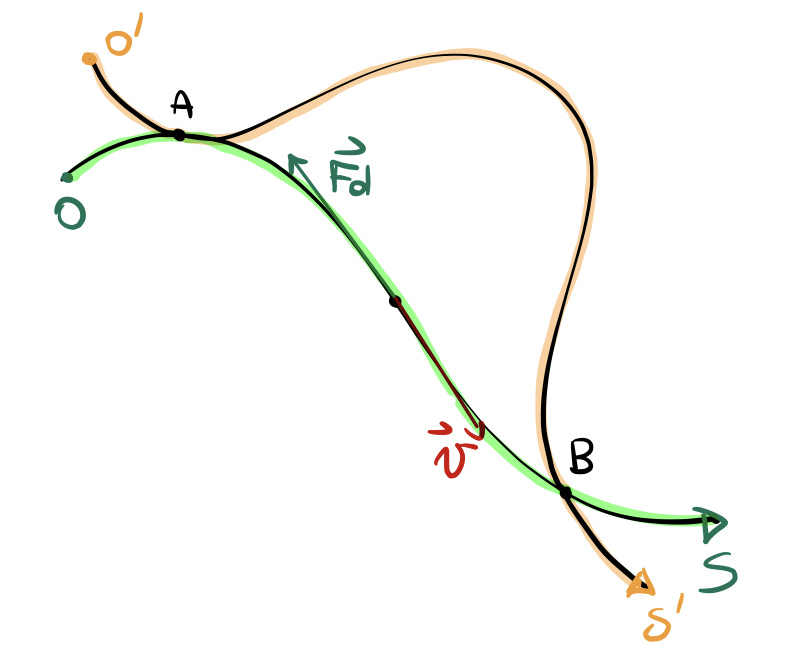
\includegraphics[width=4cm]{src/attrito dinamico.png}
        \caption{La situazione della dimostrazione}
    \end{figure}
    Supponiamo $\mu_d$ e $|\vec N|$ costanti. Ricordiamo che nella \eqref{eq: attrito  concorde} con $\d s$ si intende la coordinata curvilinea e non il vettore spostamento, di conseguenza
    \[L_s = \mu_d|\vec N|\int_A^B \d s =\mu_d|\vec N| (s_B - s_A)\]
    \[L_{s'} = \mu_d|\vec N|\int_A^B \d s' =\mu_d|\vec N| (s'_B - s'_A)\]
    Per cui i due lavori sono diversi.
\end{proof}
\subsubsection{Forza elastica}
Consideriamo il sistema in Figura \ref{fig: molla} con l'origine nella posizione di equilibrio della molla. 
\begin{figure}[h]
    \centering
    \begin{tikzpicture}
        \draw[->] (0,0)--(4,0) node [below]{$x$};
        \draw (0,0)--(0,1.5);
        \draw(0,.3)to[L, l=$k$](2,.3);
        \draw[fill=gray] (2,0)--(2.6,0)--(2.6,.6)--(2,.6)--cycle;
        \draw[dashed] (1.5,-.5)node [below]{$O$}--(1.5,1);
        \draw[dashed] (2.3,-.5)node [below]{$A$}--(2.3,1);
        \draw[dashed] (3.1,-.5)node [below]{$B$}--(3.1,1);
        \draw[latex'-latex'] (0,-.2)--node [below]{$l_0$}(1.5,-.2);
    \end{tikzpicture}
    \caption{La molla analizzata}
    \label{fig: molla}
\end{figure}
Allora, per definizione di lavoro
\[L_{AB} =\int_A^B\vec F_{el}\cdot \!\d \vec s =\int_A^B - kx\hat x\cdot \!\d x\hat x =\int_A^B - kx\d x = \left[ - \frac{1}{2} kx^2\right]_A^B =- \frac{1}{2}kx^2_B + \frac{1}{2}kx^2_A\]
\subsection{Potenziale, energia potenziale e energia meccanica}
\subsubsection{Funzione potenziale}
Una forza è conservativa se il suo lavoro non dipende dalla traiettoria, ma solo dalla posizione iniziale e finale, quindi esiste una funzione scalare $V(\vec r)$ tale che 
\[L_{AB}=V(\vec r_B)-V(\vec r_A)\]
Per trovarle è necessario fissare un origine $O$, un punto a potenziale $0$. Siccome la forza considerata è conservativa
\[L_{OB} = L_{OA} + L_{AB}\]
Da cui 
\[L_{AB} = L_{OB} - L_{OA} = V(\vec r_B) - V(\vec r_A)\]
Scegliendo un altro origine O' si ha 
\[L_{O'A} = L_{O'O} + L_{OA} = L_{O'O} + V(\vec r_A)\]
\[L_{O'B} = L_{O'O} + L_{OB} = L_{O'O} + V(\vec r_B)\]
da cui 
\[V'(\vec r) = L_{O'O} + V(\vec r)\]
La funzione potenziale è quindi definita a meno di una costante additiva. Di conseguenza 

\[\vec F\cdot \!\d \vec s = F_x\d x + F_y \d y + F_z\d z = \frac{\partial V}{\partial x}\d x + \frac{\partial V}{\partial y}\d y + \frac{\partial V}{\partial z} \d z\]
\[L_{AB} =\int_A^B\left(\frac{\partial V}{\partial x}\d x + \frac{\partial V}{\partial y}\d y + \frac{\partial V}{\partial z} \d z\right) =\int_A^B\d V\]
che è un differenziale esatto solo per le forze conservative.

\begin{lemma}[Condizione necessaria per le forze conservative]
    Se una forza è conservativa, allora è indipendente dal tempo.
\end{lemma}

\begin{lemma}[Definizione equivalente di forze conservative]
    Una forza è conservativa se e solo se
    \[\frac{\partial F_x}{\partial y} = \frac{\partial F_y}{\partial x}\qquad 
    \frac{\partial F_x}{\partial z} = \frac{\partial F_z}{\partial x}\qquad 
    \frac{\partial F_y}{\partial z} = \frac{\partial F_z}{\partial y}\]
\end{lemma}

\subsubsection{Energia potenziale e energia meccanica}
Abbiamo visto che se un punto materiale è soggetto ad una forza conservativa esiste la funzione potenziale ad essa associata. Supponiamo ora che sul corpo agisca solo questa forza. Allora per il teorema dell'energia cinetica 
\[L_{AB} = V(\vec r_B) - V(\vec r_A) = E_{c,B} - E_{c,A}\]
da cui
\[E_{c,B} - V(\vec r_B) = E_{c,A} - V(\vec r_A)\]
Introduciamo quindi una nuova quantità, l'energia potenziale associata alla forza conservativa.
\begin{boxdef}[Energia potenziale]
    Definiamo \textbf{energia potenziale} l'opposto della funzione potenziale.
    \[U(\vec r) =- V(\vec r)\]
\end{boxdef}
In modo che 
\[E_{c,B} + U(\vec r_B) = E_{c,A} + U(\vec r_A)\]
ovvero che la somma di energia potenziale e energia cinetica si conservi. Definiamo quindi 
\begin{boxdef}[Energia meccanica]
    Definiamo \textbf{energia meccanica} la somma dell'energia cinetica e di tutte le energie potenziali.
\end{boxdef}

\begin{shadedTheorem}[Conservazione dell'energia meccanica]
    Quando su un punto materiale agiscono solo forze conservative l'energia meccanica si conserva. Quando sono presenti forze non conservative, il lavoro totale delle forze non conservative è uguale alla variazione di energia meccanica.
\end{shadedTheorem}
\begin{proof}
    Dal teorema dell'energia cinetica
    \[L_{AB} = E_{c,B} - E_{c,A}\]
    separando il lavoro delle forze conservative da quello delle forze non conservative abbiamo che
    \[L_{AB}^c + L_{AB}^{nc} = E_{c,B} - E_{c,A}\]
    ma per definizione di energia potenziale
    \[U(\vec r_A) -U(\vec r_B) + L_{AB}^{nc} = E_{c,B} - E_{c,A}\]
    ovvero
    \[L_{AB}^{nc} = \left[E_{c,B} +U(\vec r_B)\right] - \left[E_{c,A} +U(\vec r_A)\right] = E_{M,B} - E_{M,A}\]
\end{proof}
\subsection{Impulso, quantità di moto e momenti}
\subsubsection{Quantità di moto}
\begin{boxdef}[Quantità di moto]
    Per una particella di massa $m$ e velocità $\vec v$ si definisce \textbf{quantità di moto} il vettore 
    \[\vec p = m \vec v\]
    Essa si misura in $kg \cdot m/s$
\end{boxdef}
Osserviamo che se siamo in un sistema inerziale e la massa è costante
\[\frac{\d\vec p}{\d t}=\frac{\d m}{\d t}\vec v+m\vec a=m\vec a = \vec F\]
Abbiamo quindi una formulazione equivalente dei principi della dinamica:

\begin{shaded}
    \begin{principio}[Conservazione della quantità di moto (Dinamica I)]
        In un \textbf{sistema di riferimento inerziale} la quantità di moto di una particella libera si conserva.
    \end{principio}
\end{shaded}

\begin{shaded}
    \begin{principio}[Dinamica II - equivalente]
        In un \textbf{sistema di riferimento inerziale}, la risultante delle forze \textbf{reali} applicate al corpo puntiforme è uguale alla derivata temporale della sua quantità di moto.
        \[\vec F =\frac{d \vec p}{dt}\]
    \end{principio}
\end{shaded}
\subsubsection{Impulso}
\begin{boxdef}[Impulso di una forza]
    Definiamo impulso di una forza $\vec F$ nell'intervallo di tempo $t_1,t_2$ il vettore
    \[\vec J_{1,2} =\int_{t_1}^{t_2}\vec F\d t\]
    esso so misura in $N\cdot s$
\end{boxdef}

\begin{shadedTheorem}[Impulso e quantità di moto]
    In un sistema di riferimento inerziale, l'impulso della forza agente su un punto materiale fra gli istanti $t_1$ e $t_2$ è pari alla variazione che la quantità di moto del punto subisce nello stesso intervallo di tempo.
    \[\vec J_{1,2} = \vec p(t_2) - \vec p(t_1)\]
\end{shadedTheorem}
\begin{proof}
    Per definizione di impulso 
    \[\vec J_{1,2} =\int_{t_1}^{t_2}\vec F\d t\]
    Ma per la formulazione equivalente del secondo principio della dinamica
    \[\vec J_{1,2} =\int_{t_1}^{t_2}\frac{\d p}{\d t}\d t = \vec p(t_2) - \vec p(t_1)\]
\end{proof}
\paragraph{Approssimazione di impulso}
Se agiscono più forze contemporaneamente, può succedere che una di esse diventi particolarmente grande nell'intervallo $t_1, t_2$. In questo caso è quindi possibile approssimare l'impulso totale a quello della singola forza impulsiva. Questa approssimazione si applica quando agiscono forze molto intense in intervalli molto brevi, ad esempio negli urti.
\subsubsection{Momento angolare e momento torcente}
\begin{boxdef}[Momento angolare o momento della quantità di moto]
     Una particella $P$ con quantità di moto $\vec p$ avrà momento angolare $\vec L_\Omega$ rispetto ad un punto $\Omega$ detto \say{polo} definito come
     \[\vec L_{\Omega} = \overrightarrow{\Omega P}\times \vec p\]
\end{boxdef}

\begin{boxdef}[Momento torcente o momento di una forza]
    Se su una particella $P$ agisce una forza $\vec F$, si dice che $\vec F$ avrà un momento $\vec \tau_\Omega$ rispetto ad un punto $\Omega$ detto \say{polo} definito come
    \[\vec \tau_{\Omega} = \overrightarrow{\Omega P}\times \vec F\]
\end{boxdef}
\begin{shadedTheorem}[Momento angolare]
    In un sistema di riferimento inerziale, se si sceglie come polo un punto $\Omega$ fisso, la risultante dei momenti della forze agenti su una particella $P$ è pari alla derivata temporale del momento angolare della particella stessa.
\end{shadedTheorem}
\begin{proof}
    Consideriamo il sistema di riferimento ortonormale $Oxyz$. Per semplicità indichiamo $\vec r:= \overrightarrow{\Omega P}$, $\vec r_{\Omega}:= \overrightarrow{O\Omega}$ e $\vec r_{P}:= \overrightarrow{OP}$
    \[
    \begin{aligned}
        \frac{\d \vec L}{\d t} &= \frac{\d}{\d t}\left( \vec r\times \vec p \right) = \frac{\d \vec r}{\d t} \times m \vec v + \vec r \times m\frac{\d \vec v}{\d t} = \frac{\d (\vec r_P -\vec r_\Omega)}{\d t} \times m \vec v + \vec r \times m\vec a = \\& = \frac{\d\vec r_P}{\d t} \times m \vec v - \frac{\d \vec r_\Omega}{\d t} \times m \vec v + \vec r \times m\vec a = \underbrace{\vec v \times m\vec v}_0 - \vec v_\Omega \times \vec p +\vec r \times \vec F = \\ &=\boxed{\vec \tau_{\Omega} - \vec v_\Omega \times \vec p}
    \end{aligned}\]
    In particolare se il polo è fisso $\vec v_\Omega=0$, quindi \[\frac{\d \vec L}{\d t} = \vec \tau_{\Omega}\]
\end{proof}
\begin{corollary*}[Conservazione del momento angolare]
    In un sistema di riferimento inerziale, se si sceglie come polo un punto fisso, il momeento angolare di una particella si conserva se e solo se la risultante dei momenti torcenti delle forze agenti su di essa è nullo.
\end{corollary*}
\begin{shadedTheorem}[Momento dell'impulso]
    In un sistema di riferimento inerziale, la variazione del momento angolare di una particella in un intervallo di tempo molto breve è uguale al momento dell'impulso applicato alla particella nello stesso intervallo.
    \[\vec L_{\Omega}(t_2) -\vec L_{\Omega}(t_1) = \vec r \times \vec J_{1,2}\]
\end{shadedTheorem}
\begin{proof}
    Si utilizza la notazione della dimostrazione precedente. Dal teorema del momento angolare 
    \[\vec \tau_\Omega =\frac{\d \vec L_{\Omega}}{\d t}\]
    Integrando nel tempo entrambi i membri, per il teorema fondamentale del Calcolo
    \[\int_{t_1}^{t_2}\vec \tau_\Omega \d t= \int_{t_1}^{t_2}\frac{\d \vec L_{\Omega}}{\d t}\d t = \vec L_{\Omega}(t_2) -\vec L_{\Omega}(t_1)\]
    Se l'intervallo di tempo è molto piccolo possiamo considerare la particella ferma, quindi $\vec r$ può essere considerato costante.
    \[\int_{t_1}^{t_2}\vec \tau_\Omega \d t = \int_{t_1}^{t_2}\vec r \times \vec F_{tot} \d t = \vec r \times\int_{t_1}^{t_2} \vec F_{tot} \d t = \vec r \times \vec J_{1,2}\]
    Da cui
    \[\vec L_{\Omega}(t_2) -\vec L_{\Omega}(t_1) = \vec r \times \vec J_{1,2}\]
\end{proof}
\section{Dinamica dei sistemi di particelle}
\subsection{Equazioni cardinali della dinamica delle particelle}
Consideriamo  un insieme di $n$ particelle di dimensione trascurabile. È fondamentale scegliere cosa considerare interno al sistema e cosa esterno.
\begin{boxdef}
    [Forze interne e esterne]
    Si dicono \textbf{forze interne} le forze genreate da corpi interni al sistema e \textbf{forze esterne} le forze generate da oggetti esterni al sistema.
\end{boxdef}
per semplicità si omettono i simboli di vettore e la specifica del polo a pedice dei momenti (si sottintende che il polo sia $\Omega$).
\begin{table}[h]
    \centering
    \everymath{\scriptstyle}
    \begin{tabular}[h]{|c|c|c|}
        \hline
        \textbf{Descrizione}&\textbf{Relativo alla singola particella}& \textbf{Totale del sistema}\\\hline
        Risultante delle forze esterne & $f^e_i$ & $F^e= \sum_if^e_i$\\
        Risultante delle forze interne & $f^i_i$ & $F^i = \sum_i f^i_i$\\
        Quantità di moto & $p_i$ & $P = \sum_i p_i$ \\
        Momento torcente (forze interne)& $\tau_i^i$ & $M^i = \sum_i \tau_i^i$\\
        Momento torcente (forze esterne)& $\tau_i^e$ & $M^e = \sum_i \tau_i^e$\\
        Momento angolare & $L_i $ & $\mathcal{L}= \sum_iL_i$\\
        Lavoro (forze interne) & $W_i^i$ & $\mathcal{W}^i = \sum_i W_i^i$\\
        Lavoro (forze esterne) & $W_i^e$ & $\mathcal{W}^e = \sum_i W_i^e$\\
        Energia cinetica & $ \frac{1}{2}mv^2_i$  & $K=\sum_i \frac{1}{2}mv^2_i$\\
        \hline
    \end{tabular}
    \caption{Notazione}
\end{table}
Dalla dinamica delle singole particelle ricaviamo che 
\[\begin{cases} 
    F = ma\\
    E_{CF} - E_{CI} = W\\
    L_{NC} = \Delta E_M\\
    \tau = \frac{\d L}{\d t} + v_\Omega \times p 
\end{cases} \]
Per ogni particella abbiamo che 
\[f_i = f_i^e + f_i^i = ma = \frac{\d p_i}{\d t}\tag{i}\]
\[\tau_i =\tau_i^i + \tau_i^e =\frac{\d L}{\d t} + v_\Omega \times p_i\tag{ii}\]
\[W = W^i_i + W^e_i = \frac{1}{2}m_iv_{i,f}^2 - \frac{1}{2}m_iv_{i,i}^2\tag{iii}\]
Adesso sommiamo su tutte le particelle
\begin{itemize}
    \item forze
    \[\sum_if_i = \sum_if_i^e + \sum_if_i^i = \sum_i \frac{\d p_i}{\d t} =\frac{\d }{\d t}\left(\sum_ip_i\right)\]
    \[F^e + F^i =\frac{\d P}{\d t} \tag{I}\]
    \item momenti
    \[\sum_i\tau_i =\sum_i\tau_i^i + \sum_i\tau_i^e =\sum_i\frac{\d L}{\d t} + \sum_iv_\Omega \times p_i = \frac{\d L_i}{\d t} + v_\Omega \times \sum_ip_i \]
    \[M^i + M^e =\frac{\d \mathcal{L}}{\d t} + v_{\Omega} \times P \tag{II}\]
    \item lavori
    \[\sum_iW = \sum_iW^i_i + \sum_iW^e_i = \sum_i\frac{1}{2}m_iv_{i,f}^2 - \sum_i\frac{1}{2}m_iv_{i,i}^2\]
    \[\mathcal{W}^i +\mathcal{W}^e = K_f - K_i\tag{III}\]
\end{itemize}
\begin{shaded}
\begin{principio}[Dinamica III - sistemi]
    In un sistema di riferimento inerziale la quantità di moto totale e il momento angolare totale rispetto ad un polo fisso di un sistema libero si conservano.
\end{principio}
\end{shaded}
Per le ipotesi del terzo principio supponiamo $F^e=0$ e $v_\Omega=0$. Allora
\begin{equation}\begin{cases} 
    \cancel{F^e} + F^i =\cancel{\frac{\d P}{\d t}}\\
    M^i + \cancel{M^e} = \cancel{\frac{\d \mathcal{L}}{\d t}} + \cancel{v_{\Omega} \times P}\\
    \mathcal{W}^i + \cancel{\mathcal{W}^e} = K_f - K_i\
\end{cases} \implies
\begin{cases} 
    F^i = 0\\
    M^i = 0\\
    \mathcal{W}^i= K_f - K_i\
\end{cases} 
\label{eq: conseguenze dinamica 3}
\end{equation}
Inoltre si ricava che anche se cade l'ipotesi per cui il sistema deve essere libero, si ha comunque il sistema \eqref{eq: conseguenze dinamica 3}. Questo porta quindi ad una semplificazione delle equazioni I, II e III, ovvero alle \textbf{equazioni cardinali della dinamica delle particelle}:
\begin{equation}
    \renewcommand{\arraystretch}{2.5}
    \left\{\begin{array}{ll} 
        F^e =\frac{\d P}{\d t}\\
        M^e = \frac{\d \mathcal{L}}{\d t} & \text{con $\Omega$ fisso}
     \end{array} \right.
     \label{eq: cardinali}
\end{equation}
Si dimostra inoltre che il terzo principio della dinamica dei sistemi è equivalente al principio di azione e reazione:
\begin{proof}
    Siano $P_1$ e $P_2$ due particelle. Per il principio di azione e reazione $f_{12}=-f_{21}$ sono dirette lungo la congiungente. Dalle equazioni \eqref{eq: conseguenze dinamica 3} \begin{itemize}
        \item $F_i=0$, quindi $f_{12}+f_{21}=0$, per cui $f_{12}=-f_{21}$
        \item $M^i=0$, quindi scegliamo un polo $\Omega$ qualsiasi e chiamiamo $\vec r_1 = \overrightarrow{\Omega P_1}$ e $\vec r_2 = \overrightarrow{\Omega P_2}$. Segue che
        \[\tau_1 +\tau_2 = 0\quad\Harr\quad  r_1 \times f_{21} + r_2 \times f_{12} = 0\quad \Harr\quad (r_1 - r_2) \times f_{12} = 0\quad \Harr\quad r_{12} \times f_{12} = 0 \quad \Harr\quad f_{12}\parallelo r_{12}\]
    \end{itemize}
\end{proof}
\subsection{Centro di massa}
\begin{boxdef}[Centro di massa]
    Dote $n$ particelle di cui conosciamo la massa $m_i$ e la posizione $\vec r_i$ si definisce centro di massa del sistema il punto $C_M=O+\vec r_{CM}$ tale che 
    \[\vec r_{CM} =\frac{~~\sum\limits_{i = 1}^nm_i\vec r_i~~}{\sum\limits_{i = 1}^nm_i}\]
\end{boxdef}
\subsubsection{Equazioni cardinali e centro di massa}
\label{sss: eq cardinali e cdm}
\begin{shadedTheorem}[Centro di massa]
    Il centro di massa di un sistema con massa $\mathcal M$ costante si muove come una particella in cui è concentrata tutta la massa del sistema e è applicata una forza pari alla risultante delle forze esterne agenti sul sistema stesso.
\end{shadedTheorem}
\begin{proof}
Consideriamo la definizione di centro di massa. Osserviamo che a denominatore compare la massa totale del sistema $\mathcal{M}= \sum\limits_{i = 1}^nm_i$. Moltiplicando ad entrambi i membro per $\mathcal{M}$ otteniamo
\[\mathcal{M} \vec r_{CM} = \sum\limits_{i = 1}^nm_i\vec r_i\]
Derivando nel tempo
\[\frac{\d}{\d t}\left(\mathcal{M} \vec r_{CM}\right) =\mathcal{M}\vec v_{CM}
= \frac{\d}{\d t}\left(\sum\limits_{i = 1}^nm_i\vec r_i \right) =
 \sum\limits_{i = 1}^n\left(m_i \frac{\d \vec r_i}{\d t} \right) = \sum\limits_{i = 1}^nm_iv_i= P\]
Osserviamo quindi che la quantità di moto totale del sistema $P$ è quella che avrebbe una particella di massa pari alla massa totale del sistema che si muove con la velocità del centro di massa. 

Derivando ancora rispetto al tempo otteniamo 
\[\frac{\d}{\d t}\left( \mathcal{M}\vec v_{CM} \right) = \frac{\d P}{\d t} = F^e\]
\begin{equation}F^e = \mathcal{M} \vec a_{CM}\end{equation}
ovvero l'equazione del moto del centro di massa.
\end{proof}

Riprendiamo l'equazione (II). Abbiamo quindi che 
\[M^e = \frac{\d \mathcal L}{\d t} + v_\Omega \times P\]
poniamo ora $\Omega \equiv C_M$, allora siccome $P=\mathcal M v_{CM}$, si ricava
\[v_{CM} \times P= v_{CM} \times \mathcal M v_{CM} = 0\]
Da cui abbiamo la formulazione completa delle equazioni cardinali della dinamica dei sistemi:
\begin{shaded}
\begin{equation}
    \renewcommand{\arraystretch}{2.5}
    \left\{\begin{array}{ll} 
        F^e =\frac{\d P}{\d t}\\
        M^e = \frac{\d \mathcal{L}}{\d t} & \text{con $\Omega$ fisso o $\Omega \equiv C_M$}
     \end{array} \right.
     \label{eq: cardinali - rev}
\end{equation}
\end{shaded}
\subsection{Urti e esplosioni}
Si dice urto un interazione molto breve e molto intensa tra due particelle in cui si sviluppano forze impulsive. 
Possiamo quindi assumere che durante l'urto le posizioni rimangano invariate, per cui le energie potenziali non cambiano subito prima e subito dopo l'urto.
Se all'istante $t=0$ avviene l'urto e le particelle sono libere $J_{imp}^e=0$, per cui
\[J_{imp}^e = \int_{0^ - }^{0^ + }F^e\d t =\int_{0^ -}^{0^ +}\frac{\d P}{\d t} \d t= P(0^ +) - P(0^ -) = 0\]
la quantità di moto totale del sistema si conserva. Se invece il sistema non è libero
\[J_{imp}^e =\Delta P\]
Analogamente, se il sistema è libero da forze impulsive esterne il momento angolare si conserva, mentre se sono presenti forze impulsive esterne, il momento dell'impulso totale è uguale alla variazione del momento angolare
\[\sum_{i = 1}^n\vec r_i \times \vec j_i = \Delta \mathcal L\]
Se il sistema è vincolato, è possibile che i vincoli possano dare luogo a forze impulsive esterne: la quantità di moto si conserva solo nelle direzioni in cui la risultante delle forze impulsive esterne è nulla.
\subsubsection{Classificazione degli urti}
Proponiamo ora una breve classificazione degli urti in base alla variazione di energia durante l'urto.
\begin{itemize}
    \item \textbf{Urti perfettamente elastici:} durante l'urto si conserva l'energia cinetica totale
    \[\Delta E_c = 0\]
    \item \textbf{Urti perfettamente anelastici:} al termine dell'urto le particelle che si sono scontrate rimangono unite. Non si conserva l'energia cinetica. \[\Delta E_c < 0\]
    \item \textbf{Esplosione:} un corpo si separa in più pezzi (un urto anelastico ma con il tempo al contrario). C'è un aumento di energia cinetica totale.
    \[\Delta E_c > 0\]
\end{itemize}
\subsection{Energia meccanica in un sistema di particelle}
Abbiamo dimostrato precedentemente che 
\[K_f - K_i = \mathcal W^e + \mathcal W^i\]

Se tutte le forze interne ed esterne sono conservative, per ogni particella si ha
\[W^e_i+ W^i_i =-\Delta U_i^i -\Delta U_i^e\]
dove $\Delta U_i$ è la variazione di energia potenziale sulla singola particella $i-$esima. Sommando su tutte le particelle (definiamo $\scriptstyle \Delta \mathcal U = \sum_i\Delta U_i= \mathcal U_f-\mathcal U_i$)
\[\sum_iW_i^i +\sum_iW_i^e = \sum_i( -\Delta U_i^i) + \sum_i( -\Delta U_i^e)\]
\[K_f - K_i =\mathcal W^i +\mathcal W^e = -\Delta \mathcal U^i - \Delta \mathcal U^e = \mathcal U_i^e +\mathcal U_i^i - \mathcal U_f^e-\mathcal U_f^i\]
\[\mathcal{E}_M: = K_f +\mathcal U_f^e +\mathcal U_f^i = K_i +\mathcal U_i^e +\mathcal U_i^i\]
\begin{shadedTheorem}[Conservazione energia meccanica]
    Se su un sistema agiscono solo forze conservative (interne ed esterne), allora l'energia meccanica si conserva.
\end{shadedTheorem}
Analogamente, se compaiono forze non conservative
\[K_f - K_i = \mathcal W^e_{C} + \mathcal W^i_C + \mathcal W^e_{NC} + \mathcal W^i_{NC}\]
Per le forze conservative vale ancora 
\[\mathcal W^i_C +\mathcal W^e_C = -\Delta \mathcal U^i - \Delta \mathcal U^e = \mathcal U_i^e +\mathcal U_i^i - \mathcal U_f^e-\mathcal U_f^i\]
Quindi
\[\mathcal{E}_{M,f} -\mathcal{E}_{M,i} =\underbrace{K_f +\mathcal U_f^i + \mathcal U_f^e} - \left( \underbrace{K_i -\mathcal U_i^i -\mathcal U_i^e} \right) = \mathcal W_{NC}^e +\mathcal W_{NC}^i\]
\subsection{Il sistema di riferimento del centro di massa}
Consideriamo un sistema di riferimento in cui l'origine coincide con il centro di massa e i cui assi hanno un'orientazione costante rispetto al sistema di riferimento inerziale $Oxyz$. Indichiamo con un apice le grandezze relative al sistema di riferimento $C_Mx'y'z'$ del centro di massa.

Osserviamo la quantità di moto dal sistema $C_Mx'y'z'$. Abbiamo ricavato precedentemente che $v_i=v_{CM}+v_i'$. Di conseguenza, moltiplicando per le masse e sommando su tutte le particelle ricaviamo che 
\[P' =\sum_im_iv_i' = \sum_im_iv_i - \mathcal M v_{CM} = 0 \]
per quanto discusso al punto \ref{sss: eq cardinali e cdm}. Di conseguenza la quantità di moto totale del sistema rispetto al sistema di riferimento del centro di massa è sempre nulla.
\subsubsection{Teoremi di König}
\begin{shadedTheorem}[König - energia cinetica di un sistema di particelle]
    In un sistema di riferimento inerziale l'energia cinetica di un sistema materiale può essere espressa come la somma dell'energia cinetica che il sistema avrebbe se tutta la sua massa fosse concentrata nel centro di massa con velocità pari a quella del centro di massa stesso, più l'energia cinetica del sistema nel sistema di riferimento del centro di massa.
    \[K =\frac{1}{2}\mathcal M v_{CM}^2 + K'\]
\end{shadedTheorem}
\begin{proof}
    \[\begin{aligned}K &=\sum_i \frac{1}{2}m_iv_i^2 = \sum_i \frac{1}{2}m_i(v_{CM} + v_i')^2 = \sum_i \frac{1}{2}m_iv_{CM}^2 +\sum_i \frac{1}{2}m_iv_i'^2 + \sum_im_iv_{CM}\cdot v_i' = \\&= \frac{1}{2}\mathcal M v_{CM}^2 + K' + v_{CM}\cdot \underbrace{\sum_im_iv_i'}_{ =P' = 0}
    = \boxed{\frac{1}{2}\mathcal M v_{CM}^2 + K} \end{aligned}\]
\end{proof}
\begin{shadedTheorem}[König - momento angolare di un sistema di particelle]
    In un sistema di riferimento inerziale il momento angolare di un sistema materiale può essere espresso come la somma del momento angolare che il sistema avrebbe se tutta la sua massa fosse concentrata nel centro di massa con velocità pari a quella del centro di massa stesso, più il momento angolare del sistema rispetto al centro di massa usato come polo.
    \[\vec L_O = \vec r_{CM} \times \mathcal M \vec v_{CM} + \vec L_{CM}\]
\end{shadedTheorem}
\begin{proof}
    Scegliamo come polo l'origine $O$ del sistema di riferimento inerziale.
    \[\begin{aligned}
        L_O &= \sum_i r_i \times m_iv_i = \sum_i (r_{CM} + r_i') \times m_i(v_{CM} + v'_i) = \\&=
        r_{CM} \times v_{CM}\underbrace{\sum_i m_i}_{\mathcal M} +
        r_{CM} \times \underbrace{\sum_i m_iv_i}_{ = P = 0} +
        \underbrace{\sum_i m_i r_i' }_{ =r'_{CM} = 0}\times v_{CM} +
        \underbrace{\sum_i r_i' \times m_iv_i}_{L_{CM}} =\\&= \boxed{\vec r_{CM} \times \mathcal M \vec v_{CM} + \vec L_{CM}}
    \end{aligned}\]
\end{proof}
\section{Elementi di meccanica di sistemi rigidi semplici}
\begin{boxdef}[Corpo rigido]
    Un corpo rigido è un sisetma materiale indeformabile. Può essere schematizzato da un sistema di punti materiali a distanza fissata.
\end{boxdef}
Un corpo rigido non vincolato è un sistema a sei gradi di libertà, ovvero la sua posizione tridimensionale è univocamente determinata da 6 coordinate.
\\
Preso un punto $P$ qualsiasi (spesso conviene scegliere il centro di massa) e un asse qualsiasi solidale al corpo rigido\begin{itemize}
    \item 3 coordinate cartesiane indicano la posizione di P
    \item 2 angoli specificano l'orientazione dell'asse
    \item 1 angolo specifica la rotazione del corpo rigido attorno all'asse.
\end{itemize}

Se in un certo istante il corpo rigido sta ruotando con velocità angolare $\vec\omega$ la velocità di un generico punto $P$ può essere espressa nella forma 
\[\vec v_P =\vec v_{CM} +\vec\omega \times \vec r_{P}'\]
Osserviamo quindi che un corpo rigido è un sistema che rototrasla, tuttavia il sistema di riferimento del centro di massa trasla solamente, mentre nel sistema di riferimento del centro di massa il corpo ruota solamente.
\paragraph{Condizioni di equilibrio}
Un corpo rigido è in equilibrio se la risultante delle forze esterne è nulla e il momento risultante dei momenti esterni è nullo (relativamente ad un polo fisso o al centro di massa).

\subsection{Momento di inerzia}
Supponiamo un manubrio che ruota nel piano $yz$ con velocità angolare $\vec \omega=\omega \hat x$ perpendicolare al manubrio. Indichiamo con $d_1$ la distanza della particella di massa $m_1$ dal centro di massa e con $d_2$ la distanza della particella di massa $m_2$ dal centro di massa.
Allora
\[v_1' =\vec\omega \times \vec d_1\qquad v_2' =\vec\omega \times \vec d_2\]
Inoltre, per il teorema di König (II) 
\[\vec L_O = \vec r_{CM} \times \mathcal M \vec v_{CM} + \vec L_{CM}\]
Di conseguenza
\[\vec L_{CM} = \sum_ir_i' \times m_iv_i' = d_1m_1\omega d_1\hat x + d_2m_2\omega d_2\hat x = \left( m_1d_1^2 + m_2d^2_2 \right)\omega \hat x = I\vec \omega\]
Definiamo quindi il momento di inerzia
\begin{boxdef}[Momento di inerzia]
    Definiamo momento di inerzia rispetto ad un asse perpendicolare al manubrio e passante per il centro di massa la quantità
    \[I_{CM} = m_1d_1^2 + m_2d_2^2\]
\end{boxdef}
Inoltre, se deriviamo l'equazione precedente nel tempo
\[\vec M_{CM}^e\frac{\d L_{CM}}{\d t} = \frac{\d}{\d t}\left( I_{CM} \vec \omega\right) = I_{CM} \frac{\d \vec \omega}{\d t} = I_{CM}\vec \alpha\]
Analogamente per l'energia ricaviamo che 
\[K' = \sum_i \frac{1}{2}m_i\vec v_i'^2 = \frac{1}{2} m_1(\omega d_1)^2 + \frac{1}{2} m_2(\omega d_2)^2 = \frac{1}{2} \left( m_1 d_1^2 + m_2d_2^2 \right)\omega^2 = \frac{1}{2}I_{CM}\omega^2\]

\subsection{Intervento di impulsi esterni}
L'intervento di forze impulsive esterme modifica la quantità di moto totale del corpo rigido (quindi quella del centro di massa). Per il teorema dell'impulso e della quantità di moto, infatti
\[\vec J^e = \vec P(0^ +) - \vec P(0^ -)\]
. Inoltre può produrre anche variazioni del momento angolare, infatti dal teorema del momento dell'Impulso
\[\sum_i\vec r_i \times \vec j_i^e = \vec L(0^ +) - \vec L(0^ -)\]

\section{Attrazione gravitazionale}
Nel 1686 Isaac Newton osservando il moto della Luna e dei gravi posti in prossimità della superficie terrestre elaborò la legge di gravitazione universale:
\begin{shaded}
    \begin{law}[Gravitazione universale]
    Due corpi di masse $m_1$ e $m_2$ posti rispettivamente nelle posizioni $\vec r_1$ e $\vec r_2$ esercitano l'uno sull'altro delle forze attrattive del tipo
    \begin{eqnarray*}\vec F_{1} = - G\frac{m_1m_2}{r_{12}^2}\hat r_{12}&~~~~~~~&\vec F_2=-\vec F_1\end{eqnarray*}
    Dove $G\approx 6.67\cdot 10^{-11}N\cdot m^2\cdot kg^{-2}$ è la costante di gravitazione universale.
\end{law}
\end{shaded}
Tutte le prove sperimentali compiute finora hanno mostrato come la massa inerziale che compare nel secondo principio della dinamica e la massa gravitazionale che compare nella legge di gravitazione universale coincidono con un errore di $10^{-15}$.
\subsection{Energia potenziale gravitazionale}
Considerimamo un sistema di riferimento in coordinate polari in cui la massa $M$ si trova nell'origine. 
\[L_{AB} =\int_A^B - G\frac{m_1m_2}{r_{12}^2}\hat e_r\cdot \!\d s =  \int_A^B - G\frac{m_1m_2}{r_{12}^2}\d r = - GMm\int_A^B\frac{\d r}{r^2} = GMm\left( \frac{1}{r_B} -\frac{1}{r_A} \right)\]
Abbiamo dimostrato che il lavoro non dipende dalla traiettoria, per cui la forza è conservativa. Di conseguenza è possibile definire un energia potenziale:
\[U(r) = - \frac{GMm}{r}\]
In questo modo non esiste un punto in cui l'energia potenziale sia nulla, scegliamo di fare in modo che sia nulla quando le masse si trovano ad una distanza infinita. 

Osserviamo inoltre che la forza gravitazionale ha momento torcente nullo perché è sempre parallela al raggio, per cui il momento angolare si conserva sempre. Di conseguenza essa dà origine ad un moto piano.
\subsubsection{Velocità di fuga}
Dire che un oggetto sfugge all'attrazione gravitazionale terrestre significa affermare che arrivi così lontano che l'energia potenziale gravitazionale si annulli con velocità nulla (caso minimo)
\[\frac{1}{2} mv^2_f -\frac{GMm}{r} = \frac{1}{2}mv^2_{\infty}\]
\[\implies\quad v_f =\sqrt{\frac{2GM}{r} }\]
Che per un oggetto che parte dalla superficie terrestre è di circa $11,2 \;km/s$

%%%%%%%%%%%%%%%%%%%%%%%%%%%%%%%%%%%%%%%%%%%%%%%%%%%%%
\end{document}